\documentclass[12pt,  openany]{book}
\pagestyle{plain}
\usepackage[utf8]{inputenc}
\usepackage[T1]{fontenc}

\usepackage{extsizes}
\usepackage[english,russian]{babel}
\usepackage{geometry}
\usepackage{graphicx}
\usepackage{float}
\usepackage{csquotes}
\usepackage{hyphsubst}
\usepackage{svg}
\usepackage{tempora}
\usepackage{hyperref}
\usepackage{amsmath}
\usepackage{relsize}
\usepackage{listings}
\usepackage[nottoc,notlot,notlof,numbib]{tocbibind}
\usepackage{natbib}
\usepackage{indentfirst}
\usepackage{titlesec}
\titleformat{\chapter}[display]
  {\normalfont\bfseries}{}{0pt}{\Huge}
\usepackage{listings}
\usepackage{xcolor}
\usepackage{hyperref}
\hypersetup{
    colorlinks,
    citecolor=black,
    filecolor=black,
    linkcolor=black,
    urlcolor=black
}

\definecolor{codegreen}{rgb}{0,0.6,0}
\definecolor{codegray}{rgb}{0.5,0.5,0.5}
\definecolor{codepurple}{rgb}{0.58,0,0.82}
\definecolor{backcolour}{rgb}{0.98,0.98,0.98}

\lstdefinestyle{mystyle}{
    frame=single,
    aboveskip=5mm,
    belowskip=5mm,
    backgroundcolor=\color{backcolour},   
    commentstyle=\color{codegreen},
    keywordstyle=\color{blue},
    numberstyle=\small\color{codegray},
    stringstyle=\color{codepurple},
    basicstyle=\ttfamily\footnotesize,
    breakatwhitespace=false,         
    breaklines=true,                 
    captionpos=b,                    
    keepspaces=true,                 
    numbers=left,                    
    numbersep=7pt,                  
    showspaces=false,                
    showstringspaces=false,
    showtabs=false,                  
    tabsize=2
}

\lstset{style=mystyle}
  
\geometry{
    a4paper,
    left=30mm,
    top=20mm,
    right=15mm,
    bottom=20mm
}
\linespread{1.5}
\setlength{\parindent}{1.25cm}

\renewcommand*{\maketitle}{
\begin{titlepage}
  \begin{center}
    Федеральное государственное автономное образовательное учреждение\break высшего образования\par
    <<Московский физико-технический институт (государственный университет)>>\par
    Физтех-школа прикладной математики и информатики\par
    Кафедра банковских информационных технологий\par
  \end{center}
%
  {\bf Направление подготовки}: 01.03.02 Прикладная математика и информатика\newline
  {\bf Направленность (профиль) подготовки}: Прикладная математика и компьютерные науки\par
%
  {
    \topskip0pt
    \vspace*{\fill}
    \begin{center}
      {\bf\LARGE Проверка консистентности и изоляции транзакций в распределенных системах}\par
      (бакалаврская работа)
    \end{center}
    \vspace*{\fill}
  }
%
  \hfill
  \begin{minipage}[t]{7cm}
    {\bf Студент: \newline}
    Исаева Анна Олеговна\newline
    \vspace{-3mm}
    \rule{7cm}{0.15mm}
    \centerline{\small\it (подпись студента)}\newline
    {\bf Научный руководитель: \newline}
    Звонов Денис Владимирович\newline
    \vspace{-3mm}
    \rule{7cm}{0.15mm}
    \centerline{\small\it (подпись научного руководителя)}
  \end{minipage}
    \vspace*{\fill}
    \begin{center}
      Москва 2021
    \end{center}
\end{titlepage}
}

\begin{document}
\chapter{Аннотация}

\par Одной из составных частей компьютерных программ являются базы данных. Для обеспечения масштабируемости и надежности базы данных делают распределенными. При использовании распределенных баз данных возникает вопрос, удовлетворяют ли они заявленным характеристикам и свойствам. Это связано с проблемой обеспечения изолированности транзакций --- важнейшего инструмента взаимодействия с базой данных.
\par Тестирование распределенных систем --- нетривиальная задача, потому что ошибки сложно обнаружить, так как они зачастую являются результатом сочетания маловероятных событий. Поэтому тестирование изолированности --- это актуальный вопрос для разработчиков распределенных систем. Один из инструментов для проверки изоляции транзакций, который практически не имеет аналогов --- это инструмент хаос-тестирования Jepsen.
\par В этой работе изучен инструмент хаос-тестирования Jepsen.  Рассмотрены различные феномены, указывающие на нарушения гарантии изолированности, и которые вспомогательный инструмент Jepsen Elle может находить. Кроме того, проведено исследование база данных Azure Cosmos DB с помощью Jepsen.  В работе проанализированы найденные аномалии на соответствие заявленным моделям согласованности.

\setcounter{page}{2}
\tableofcontents
\clearpage

\chapter{Введение}

Изолированность транзакций в базах данных --- это важное свойство. Нарушение этого свойства может привести к ошибкам системы, работающей с базой данных.  Большинство распределенных систем стремятся к достижению баланса между временем выполнения операций и гарантиями изолированности операций. 
\par Тестирование может помочь в нахождении ошибок. Однако это сложный и кропотливый процесс, потому что зачастую ошибки вызываются маловероятным сочетанием событий, приводящим к нарушениям в заявленной модели согласованности. Один из инструментов для проверки соблюдения изолированности --- это инструмент хаос-тестирования Jepsen.   
\par Хаос-тестирование --- это тестирование путем внесения в систему незапланированных сбоев \cite{chaosTesting}.  Наблюдая за поведением системы, можно понять, как сделать распределенную систему более надежной. Хаос-тестирование --- это важная часть тестирования, потому что помогает выявить состояния гонки (\textit{race condition}), которые сложно иначе обнаружить в процессе разработки. Удобный инструмент для тестирования соответствия заявленной модели согласованности может существенно помочь на этапе разработки распределенной системы, возможно, стать одним из этапов CI/CD процесса.

\section{Цели работы}
\begin{itemize}
  \item Научиться применять инструмент проверки свойств транзакций Jepsen;
  \item Проанализировать с помощью выбранного инструмента реальную базу данных Azure Cosmos DB, которая еще не была исследована;
  \item Сравнить модель согласованности, заявленную в документации, и модель согласованности, установленную с помощью тестов.
\end{itemize}

\section{Основные понятия}

\emph{Параллельная система} --- это система, состоящая из независимых компонент, которые могут выполнять некоторые операции одновременно.

\emph{Распределенная система} --- это тип параллельных систем, который представляет собой систему с несколькими независимыми компонентами, расположенными на разных узлах в компьютерной сети. Эти узлы способны обмениваться данными, а также они координируют свои действия так, чтобы для конечного пользователя распределенная система работала как единая согласованная система. Система имеет логическое состояние, которое меняется с течением времени.

\emph{Хаос-тестирование \cite{chaosTesting}} --- это тестирование путем внесения в распределенную систему незапланированных сбоев.

\emph{Процесс} --- это логически однопоточная программа, которая способна выполнять некоторые операции.

\emph{Операция} --- переход из одного состояние в другое.

\emph{Атомарная операция} --- \cite{habrAtomicOperation} операция в параллельном программировании, выполняющаяся в общей области памяти потоков и завершающаяся за один шаг относительно других потоков, которые имеют доступ к этой же области памяти.  Пока атомарная операция выполняется, ни один поток не может наблюдать частичные, незафиксированные изменения. Неатомарные операции не дают такой гарантии. 

\emph{Параллелизм} --- это свойство системы, которое означает, что несколько процессов могут выполняться в одно и то же время.

\emph{Сбой} --- это состояние процесса, в котором тот не может вызывать никаких операций. 

\emph{История} --- совокупность операций и их параллельной структуры. В этой работе будут рассматриваться истории с точки зрения Jepsen. То есть истории будут представлены в виде упорядоченного списка операций вызова и завершения.

\emph{Модель согласованности} --- набор гарантий, используемый в той или иной распределенной системе для обеспечения согласованности данных.  Другими словами,  \textit{модель согласованности} --- это набор историй, которые считаются корректными с точки зрения данной распределенной системы.  Если сказано, что история нарушает какую-то модель согласованности, это означает, что история не входит в соответствующий набор историй. \cite{jepsenConsistencyModels}

\emph{Транзакция} --- некоторый конечный набор операций, переводящий данные из одного согласованного состояния в другое. Либо будет выполнена каждая операция из набора, либо ни одной.

\emph{ACID} --- основные свойства транзакций: атомарность, согласованность, изолированность и прочность.

\emph{Согласованность} --- свойство транзакций, которое гарантирует, что каждая успешно завершенная транзакция фиксирует результат, являющийся допустимым с точки зрения внутренних правил базы данных. Когда же какая-то транзакция пытается записать несогласованные данные, вся транзакция откатывается, транзакция завершается с ошибкой.

\emph{Изоляция} --- свойство транзакций, которое гарантирует, что параллельно исполняющиеся транзакции не влияют на результаты друг друга. 

\emph{Отношение <<произошло до>>(англ. \textit{happens before})} --- \cite{habrMemoryModel} это отношение между результатами двух операций.  Пусть операцию А исполняет поток X, и операцию B исполняет поток Y. Если операция A <<произошла до>>(\textit{happens-before}) операции B, то все изменения, совершенные X до операции A, и изменения, выполненные этой операцией, видимы для потока Y в момент выполнения операции B и после.  

\chapter{Основные теоретические сведения}
В этой главе будут рассмотрены основные теоретические сведения, которые будут полезны в практической части.

\par База данных --- организованная в соответствии с определёнными правилами и поддерживаемая в памяти компьютера(или нескольких компьютеров) совокупность данных, характеризующая актуальное состояние некоторой предметной области и используемая для удовлетворения информационных потребностей пользователей \cite{db}.  В данной работе будут рассматриваться распределенные базы данных, то есть таких базы данных,  которые хранят некоторые части своих данных в различных физических локациях.
\par Некоторые базы данных реализуют различные модели согласованности, позволяющие регулировать гарантии, предоставляемые базой данных. Далее будет рассмотрена наиболее часто встречаемая модель согласованности, реализуемая различными базами данных, в том числе Azure Cosmos DB.

\section{Изоляция моментальных снимков (англ.  \textit{Snapshot Isolation})\cite{jepsenConsistencyModels}}
Изоляция моментальных снимков --- это транзакционная модель. Нет гарантии доступности, то есть распределенная система может быть недоступна во время некоторых типов сетевых сбоев. Некоторые или все узлы должны приостановить работу, чтобы обеспечить безопасность.

\par Изменения транзакции видны только этой транзакции до момента фиксации, когда все изменения становятся видимыми атомарно. Если транзакция $T_1$ изменила объект \textit{x}, а другая транзакция $T_2$ совершила запись в \textit{x} после начала моментального снимка $T_1$ и до фиксации $T_1$, то $T_1$ должна прерваться.
\par
В отличие от сериализуемости(англ. \textit{Serializability}), которая обеспечивает полный порядок транзакций, изоляция моментальных снимков гарантирует только частичный порядок: подоперации в одной транзакции могут чередоваться с подоперациями из других транзакций. Наиболее заметными явлениями, допускаемыми изоляцией моментальных снимков, являются перекосы записи (англ. \textit{write skews}), которые позволяют транзакциям считывать перекрывающееся состояние, изменять непересекающиеся наборы объектов, а затем фиксировать; и аномалия транзакций только для чтения(англ.  \textit{read-only transaction anomaly}), включающая частично непересекающиеся наборы записи.
\par
Данная модель согласованности запрещает грязную запись (англ. \textit{dirty write}, $P_0$) и грязное чтение (англ.  \textit{dirty read}, $P_1$), но допустимы неповторяющееся чтение (англ. \textit{fuzzy read}, $P_2$), фантомное чтение (англ. \textit{phantom}, $P_3$)\cite{adya99:_weak_consis}. Изоляция моментальных снимков не накладывается никаких ограничений в реальном времени и не требует упорядочивания процессов между транзакциями.
\par Беренсон, Бернштейн и другие \cite {BerensonIsolationLevels} впервые определели \textit{изоляцию моментального снимка} в терминах абстрактного алгоритма: 
\begin{displayquote}
\textit{В момент начала транзакции она считывает данные из моментального снимка данных, которые были зафиксированы. Этот момент называется меткой начала отсчета. Это время может быть любым до первого чтения транзакции. Транзакция никогда не блокируется при попытке чтения до тех пор, пока данные моментального снимка из его метки начала отсчета могут быть сохранены. Записи транзакции(обновления, вставки и удаления) также будут отражены в этом моментальном снимке, чтобы их можно было считать снова, если транзакция обращается к данным во второй раз. Обновления другими транзакциями, начатыми после метки начала отсчета транзакции, невидимы для транзакции. 
\newline \newline
Когда транзакция T1 готова к фиксации, она получает метку времени фиксации, которая больше любой существующей метки начала отсчета или другой метки времени фиксации. Транзакция будет зафиксирована только в том случае, если ни одна другая транзакция T2 с меткой времени фиксации в интервале выполнения T1 [время начала отсчета, время фиксации] не записала данные, которые также записала T1. В противном случае T1 прервется. Это предотвращает потерю обновлений (англ. \textit{lost update}, P4). Когда T1 будет зафиксирована, эти изменения становятся видимыми для всех транзакций, метки начала отсчета которых больше, чем метка времени фиксации T1.
}
\end{displayquote}
\par
В другой формулировке изоляции моментальных снимков определяется как комбинация четырех свойств \cite{cerone_et_al}:
\begin{itemize}
\item внутренняя согласованность (англ. \textit{internal consistency});
\item внешняя согласованность (англ. \textit{external consistency});
\item префикс (англ. \textit{prefix}) --- здесь и далее это означает, что транзакции становятся видимыми для всех узлов в одном и том же порядке;
\item отсутствие конфликта (англ. \textit{NoConflict}) --- здесь и далее это означает, что если две транзакции изменяют один и тот же объект, одна должна быть видна другой.
\end{itemize}

\section{Граф сериализации \cite{IsolationLevelDefinitions} \cite{IsolationLevelDefinitions2}}
Сначала будут определены различные типы зависимостей, которые возникают между транзакциями, а затем через них определен \textit{граф сериализации}(\textit{\textbf{DSG}}). 
Здесь и далее $T_i/T_j$ - транзакции.
\subsection{Зависимость записи (англ. \textit{Directly Write-Depends})}
В дальнейшем будет использоваться обозначение для данного типа зависимости: \textit{ww}. Обозначение в \textit{DSG}: $T_i  \xrightarrow{\textit{ww}} T_j$
\par
Описание: $T_j$ зависит от $T_i$, когда $T_i$ устанавливает $x_i$, а $T_j$ устанавливает следующую версию \textit{x}.

\subsection{Зависимость чтения (англ. \textit{Directly Read-Depends})}
В дальнейшем будет использоваться обозначение для данного типа зависимости: \textit{wr}. Обозначение в \textit{DSG}: $T_i  \xrightarrow{\textit{wr}} T_j$
\par
Описание: $T_j$ зависит от $T_i$,  когда выполняется одно из двух условий:
\begin{itemize}
\item $T_i$ устанавливает $x_i$, $T_j$ читает $x_i$;
\item $T_i$ фиксирует изменение, а затем $T_j$ выполняет чтение на основе предикатов таким образом, что набор объектов, соответствующих предикату, изменяется фиксацией $T_i$.   Кроме того, $T_i$ --- это самая последняя транзакция, в которой было зафиксировано изменение, влияющее на соответствие $T_i$.
\end{itemize}

\subsection{Анти зависимость (англ. \textit{Directly Anti-Depends})}
В дальнейшем будет использоваться обозначение для данного типа зависимости: \textit{rw}. Обозначение в \textit{DSG}: $T_i  \xrightarrow{\textit{rw}} T_j$
\par
Описание: $T_j$ зависит от $T_i$,  когда выполняется одно из двух условий:
\begin{itemize}
\item $T_i$ считывает некоторую версию $x_i$ объекта \textit{x}, а затем $T_j$  фиксирует следующую версию \textit{x} в истории версий;
\item $T_i$ выполняет чтение на основе предикатов, а $T_j$ перезаписывает это чтение(то есть фиксирует более позднюю, следующую версию  объекта).
\end{itemize}

\subsection{Граф сериализации(англ. \textit{Direct Serialization Graph}, \textit{DSH})}
DSG имеет один узел для каждой совершенной транзакции. Направленные ребра между этими узлами представляют зависимости чтения/записи/анти. Транзакция $T_2$ зависит от $T_1$, если в графе есть путь от $T_1$ до $T_2$. 
\par
Построение DSG начинается с добавления узлов для каждой зафиксированной транзакции. Затем добавляется ребро \textit{wr}, \textit{rw} или \textit{ww} зависимости для всех пар транзакций, если выполняются условия зависимости.

\section{Феномены}
\subsection{Грязная запись (англ.  \textit{dirty write}, $P_0$) \cite{CritiqueANSI_SQL}}
Грязная запись происходит, когда одна транзакция перезаписывает значение, которое ранее было записано другой транзакцией, все еще находящейся в процессе исполнения.
\par Одна из причин, по которой грязные записи стоит избегать, заключается в том, что они влекут за собой нарушение согласованности распределенной системы.  Если на \textit{x} и \textit{y} наложено ограничение (например, $x = y$), то транзакции $T_1$ и $T_2$ соблюдают согласованность ограничения, если исполняются отдельно.  Но когда эти две транзакции исполняются вместе и изменяют \textit{x} и \textit{y} в разных порядках, то ограничение нарушается.  Такое поведение возможно только при наличии грязных записей в системе.
\par Еще одна причина необходимости защиты от грязных записей заключается в том, что без защиты от них система не может автоматически откатиться к образу <<до>> при прерывании транзакции.

\subsection{Грязное чтение (англ. \textit{dirty read}, $P_1$)}
Грязное чтение --- явление, когда одна транзакция считывает изменения, внесенные другими незафиксированными (или даже прерванными) транзакциями. \cite{sookocheff}
\par Недостаточно предотвратить только чтение значений, записанных транзакциями, которые в конечном итоге откатываются. Также необходимо предотвратить чтение значений из транзакций, которые в конечном итоге также фиксируются.  \cite{CritiqueANSI_SQL}

\subsection{Неповторяющееся чтение (англ. \textit{fuzzy read}, $P_2$)}
Неповторяющееся чтение --- это явление, которое возникает, когда значение считывается дважды во время транзакции, и эти считанные значения отличается между чтениями.  Это возможно, когда значение, считанное транзакцией, все еще находящейся в процессе исполнения, перезаписывается другой транзакцией. Даже без повторного считывания значения, которое фактически происходит, это все равно может привести к нарушению инвариантов базы данных.  \cite{CritiqueANSI_SQL}

\subsection{Фантомное чтение (англ. \textit{phantom}, $P_3$)}
Фантомное чтение происходит, когда транзакция выполняет два идентичных запроса во время обработки, но возвращаемые результаты этих двух запросов различны.  \cite{sookocheff}

\subsection{G0 (цикл записи, англ. \textit{Write Cycle})}
История содержит аномалию \textit{цикл записи}, если ее граф сериализации содержит цикл, полностью состоящий из ребер зависимости записи(\textit{ww}). 
\par Цикл записи происходит, когда две транзакции записывают один и тот же набор данных. Предотвращение циклов записи является минимальным требованием для наличия функциональной базы данных, гарантируя, что записи, выполняемые транзакцией \textit{A}, не перезаписываются транзакцией \textit{B}, пока транзакция \textit{A} все еще выполняется.  \cite{sookocheff}

\subsection{G1}
G1: включает в себя три феномена: 
\begin{itemize}
\item G1a (прерванное чтение, англ. \textit{aborted read}) --- $T_2$ считывает некоторый объект (в том числе с помощью чтения предикатов), измененный $T_1$, и $T_1$ прерывается. Чтобы предотвратить прерывание чтения, если $T_2$ читает из $T_1$ и $T_1$ прерывается, $T_2$ также должен прерваться;
\item G1b (промежуточное чтение, англ. \textit{intermediate read}) --- $T_2$ считывает версию некоторого объекта (в том числе с помощью чтения предикатов), измененную $T_1$, и это не было окончательной модификацией этого объекта $T_1$. Чтобы предотвратить промежуточное чтение, транзакции могут быть разрешены к фиксации только в том случае, если они прочитали окончательные версии объектов из других транзакций;
\item G1c (циклический информационный поток, англ. \textit{сyclic information flow}) --- граф сериализации содержит направленный цикл, полностью состоящий из ребер зависимостей (чтение и запись). Если на $T_1$ влияет $T_2$, то нет никакого пути, по которому $T_2$ также может влиять на $T_1$.
\end{itemize}

\subsection{G2-item (цикл антизависимости, англ. \textit{anti-dependency cycle})}
G2-item(anti-dependency cycle, цикл антизависимости) возникает, когда граф сериализации \textit{DSG} содержит направленный цикл, имеющий одно или несколько ребер антизависимости(\textit{rw}). 

\chapter{Методология проверки изоляции транзакций в распределенных системах}
В предыдущей главе были рассмотрены некоторые феномены, которые нарушают изоляцию транзакций в распределенной системы. Несмотря на то, что они встречаются довольно часто, их сложно обнаружить.  В этой главе будет рассмотрен инструмент, разработанный специально для проверки того, соответствует ли распределенная система и ее транзакции своим гарантиям изолированности.
\section{Jepsen}
\begin{figure}[H]
  
\includegraphics[width=\textwidth]{jepsen.jpeg}
  \caption{Схема работы Jepsen-тестирования}
\end{figure}
\par Jepsen --- это библиотека для функционального языка Clojure. Jepsen может доказать только лишь наличие ошибок, а не их отсутствие.

\par Jepsen проверяет систему, генерируя случайные последовательности операции (например, чтение, запись, cas) в распределенной системе, записывая метку времени и продолжительность каждой операции, а также создавая модель системы в памяти.  Также Jepsen может генерировать последовательности транзакций из различных операций. А затем он пытается доказать, имеет ли история событий смысл с учетом заданной модели согласованности.
\par Jepsen также может генерировать разные сбои в распределенной системе, например, проблемы с сетью, уничтожение компонентов, а также генерацию случайной нагрузки.
\par Jepsen инкапсулирует код для настройки и демонтажа распределенной системы, которую нужно протестировать. Возможно выполнить настройку и демонтаж вручную, но если позволить Jepsen справиться с этим, то возможно запускать тесты в системе \textit{CI}, параметризовать конфигурацию базы данных, запускать несколько тестов подряд с чистого листа и так далее.

\subsection{Этапы работы Jepsen}
При запуске теста jepsen сначала подключается по ssh к каждому узлу, загрузит, распакует и настроит на них распределенную систему.
\par После запускаются клиентские процессы и процессы-сбои (англ. \textit{nemesis}). Во время теста в jepsen есть два типа процессов: один --- клиент, который будет выполнять различные операции с системой (с интервалом и частотой, заданных в генераторе), а другой --- nemesis, вносящий сбои и разрушения и выполнять восстановление системы. После завершения операций jepsen будет использовать checker (после jepsen 2.0 это будет Elle), чтобы проверить правильность истории операций с определенными моделями согласованности.
\par Jepsen кластер состоит из \textit{jepsen-control} узла, который управляет другими узлами, настройкой и удалением, генерирует данные и сбои. А также из обычных узлов, далее они будут обозначаться как \textit{jepsen-nX}. 
\subsubsection{Настройка операционной системы}
Первым этапом на узлах \textit{jepsen-nX} вызывается настройка операционной системы,  которая была задана в параметрах тестирующей системы. Jepsen поддерживает несколько операционных систем: 
\begin{enumerate}
\item \textit{jepsen.os.centos}
\item \textit{jepsen.os.debian}
\item \textit{jepsen.os.smartos}
\item \textit{jepsen.os.ubuntu}
\end{enumerate}
\subsubsection{Настройка базы данных}
Далее необходимо настроить распределенную систему на узлах кластера \textit{jepsen-nX}.  Для этого специальная функция \textit{db} использует \textit{reify} для создания нового объекта, удовлетворяющего протоколу баз данных Jepsen (из пространства имен \textit{db}).  Этот протокол определяет две функции, которые должны выполнять настройку(\textit{setup!}) и демонтаж(\textit{teardown!}) узла тестирования базы данных.
\par В функции \textit{setup!} прописывается алгоритм установки базы данных на узел. Как правило, сначала загружается архив в нужными файлами, распаковывается в каталог и запускается нужный двоичный файл.
\par Для установки пакетов нужно быть в  root,  поэтому используется \textit{jepsen.control/su}, чтобы получить привилегии root.  А для загрузки и установки архива используется \textit{jepsen.control.util/install-archive!}. 
\par  Jepsen запускает установку (а после и демонтаж) одновременно на всех узлах. Это может занимать некоторое время, так как каждый узел должен загрузить архив. Но при повторных запусках Jepsen будет использовать кэшированный архив.
\par Распределенная система должна быть запущена на каждом узле в качестве демона (\textit{daemon}) в фоновом режиме. Рекомендуется использовать функции \textit{jepsen.control.util} для запуска и остановки демонов для запуска распределенной системы.

\subsubsection{Демонтаж базы данных}
Чтобы убедиться, что действия предыдущего запуска тестовой системы не влияли на текущие результаты, Jepsen выполняет демонтаж базы данных перед настройкой в начале теста.  Затем он снова выполняет демонтаж по завершении теста.  Для этого используется команда остановки демона, а после удаляются каталоги с файлами. Для этого используется \textit{jepsen.control/exec}.  Jepsen автоматически связывает \textit{exec} для работы с нужным узлом, настроенным во время \textit{db/setup!}, но при необходимости  можно подключиться к произвольным узлам.

\subsubsection{Генератор и вид операций}
\textit{Jepsen client} принимает операцию, применяет ее к тестируемой системе и возвращает соответствующие значения операции завершения.  У операций имеются поля \textit{:type}, \textit{:f}, \textit{:value}.  $:type=:invoke$ означает, что это операция только собирается быть применена к системе.  $:type=:ok$ означает, что операция завершена успешно, а $:type=:fail$ означает, что операция завершилась с ошибкой.  \textit{:f} несет в себе информацию о том, какая именно операция должна быть применена к тестируемой системе, например, \textit{read}, \textit{write}, \textit{append}.
\par Вызовы функций параметризуются их аргументами и возвращаемым значениям. Операции Jepsen параметризуются значениями \textit{:value}, которое может быть любым --- Jepsen не проверяет их. Например,  $:f=:write, :value=k$ используется, чтобы указать значение, которое записывается. А $:f=:read, :value=k$ используется, чтобы указать значение, которое (в конечном итоге) будет прочитано. Когда операция чтения только вызывается,  используется $:value = nil$, так как неизвестно, что будет прочитано.
\par \textit{jepsen.generator} генерирует операции описанного вида. И даже последовательности операций, которые должны исполняться как транзакции. 

\subsubsection{Jepsen Client}
После настройки распределенной системы на \textit{jepsen-control}  запускается генератор некоторых последовательностей операций.  Эти операции передаются на исполняющие узлы \textit{jepsen-nX}, где для их обработки определен \textit{Jepsen client}. 
\par Для этого будет определен новый тип структуры данных \textbf{Client}.  Клиенты поддерживают клиентский протокол Jepsen, и, как и \textit{reify}, предоставляют реализацию клиентских функций(\textit{open!}, \textit{setup!}, \textit{invoke!}, \textit{teardown!}, \textit{close!}), которые должны быть реализованы.  
\par Жизненный цикл клиента состоит из 5 частей. Сначала \textit{open!} получает копию клиента, привязанную к определенному узлу, и устанавливает соединение с тестируемой системой. Далее \textit{setup!} инициализирует нужные тесту структуры данных, например, создает таблицы. Затем \textit{invoke!} применяет операции, сгенерированные \textit{jepsen.generator}, к тестируемой системе и возвращает соответствующие операции завершения. Потом \textit{teardown!} удаляет и очищает все то, что было создано \textit{setup!}. И затем \textit{close!} закрывает сетевое подключение и завершает жизненный цикл клиента.

\subsubsection{Проверка корректности}
Итак, после генерации операций их выполняют клиенты. В результаты работы клиентов записываются истории. Они содержат сами операции с их результатом, а также метки времени и продолжительность каждой операции.  Дальше эти истории необходимо проанализировать. Jepsen использует модель для представления абстрактного поведения системы и средство для проверки того, соответствует ли история заданной модели.  В более старых тестах Jepsen использовался \textit{knossos.model} для проверки корректности.   Для Jepsen версии $2.0$ и выше используется \textit{Elle}. В этой работе также будет использоваться  \textit{Elle}, которая будет подробнее рассмотрена далее.
\par Также можно использовать \textit{checker/compose} для выполнения анализа линеаризуемости и создания графиков производительности. Кроме того, есть возможность создавать HTML-визуализации истории. Для этого нужно использовать \textit{jepsen.checker.timeline}.

\subsubsection{Сбои}
Для добавления сбоев в тестируемую систему используется Немезида(англ. \textit{nemesis}). Это специальный клиент, не привязанный к какому-либо конкретному узлу.  \textit{jepsen.nemesis} обеспечивает несколько встроенных режимов  сбоев.  Например, \textit{nemesis/partition-random-halves} разделяет сеть на две половины, выбранные случайным образом, а затем возвращает в исходное рабочее состояние по прошествии какого-то времени. Также можно добавлять в тестируемую систему паузы и сдвиги часов.
\par Как и для остальных клиентов, операции сбоев генерируются на узле \textit{jepsen-control} с помощью такого же генератора. 

\subsection{Формат результатов тестов Jepsen}
При каждом запуске jepsen создает новый каталог в \textit{store/} директории, и можно увидеть последние результаты в папке \textit{store/latest}. Там лежат несколько файлов.  Файл \textit{history.txt} содержит операции, которые выполнял тест.  Файл \textit{jepsen.log} --- копия консоли для этого запуска, \textit{jepsen.log} есть журнал всех операций, выполненных jepsen к тестируемой системе, и, наконец, \textit{test.fressian} --- это необработанные данные теста, включающие полную историю операций, \textit{timeline.html} --- это html документ, который показывает удобную временную шкалу операций. Эта шкала очень полезный инструмент для понимания порядка операций в тесте и выявления причин несогласованности результатов теста. Синий цвет указывает на то, что операция прошла успешно, красный --- на неудачную операцию (состояние системы не изменилось), а оранжевый --- на неопределенную операцию.

\section{Elle}
Elle --- это инструмент для анализа результатов тестирования. Он автоматически строит граф сериализации для транзакций и ищет циклы в этом графе для выявления нарушений согласованности. Например, если граф содержит цикл, то невозможно сказать, какая транзакция произошла до и после, а значит, нарушается гарантия линеаризуемости.  
Дополнительно проверяется наличие прерванных и промежуточных считываний и другие нарушения.
\par Elle не является полным: он может не идентифицировать аномалии, которые присутствовали в тестируемой системе. Это следствие двух факторов:
\begin{itemize}
\item Elle проверяет истории, наблюдаемые в реальных базах данных, где результаты транзакций могут остаться незамеченными, а информация о времени может быть не такой точной, как хотелось бы;
\item проверка сериализуемости является NP-полной задачей \cite{NP_Serializability}; Elle намеренно ограничивает свои выводы теми, которые можно решить за линейное (или \textit{log}-линейное) время.  
\end{itemize}
В зависимости от того, какие ребра содержались в найденном цикле в графе сериализации(\textit{ww}, \textit{wr} или \textit{rw}), делается вывод о том, какая найдена аномалия.
\subsection{Список возможных аномалий}
\begin{itemize}
\item G0 (цикл записи, англ. \textit{Write Cycle}); 
\item G1a (прерванное чтение, англ. \textit{aborted read});
\item G1b (промежуточное чтение, англ. \textit{intermediate read});
\item G1c (циклический информационный поток, англ. \textit{сyclic information flow});
\item G-single (перекос чтения, англ. \textit{read skew});
\item G2-item (цикл анти зависимости, англ.  \textit{anti-dependency cycle}).
\end{itemize}
\par Инструмент также умеет проверять согласованность внутри одной транзакции: то есть можно проверить, что транзакции считывают значения, соответствующие их собственным предыдущим записям, нет дублирующихся элементов и неожиданных элементов (например, элементов, которые никогда не были записаны).

\chapter{Исследование согласованности Azure Cosmos DB}
\section{Azure Cosmos DB}
Azure Cosmos DB - это коммерческий (с закрытым исходным кодом) глобально распределенный многомодельный сервис баз данных Microsoft <<для управления данными в планетарном масштабе>>, запущенный в мае 2017 года. Он не зависит от схемы, горизонтально масштабируем и обычно классифицируется как база данных NoSQL.
\par Cosmos DB поддерживает 5 API: Table, SQL, MongoDB, Gremlin, Cassandra.  Тут SQL --- это документно ориентированный API, называющийся раньше \textit{DocumentDB}, и имеет ряд существенных отличий по сравнению с традиционными реляционными базами данных.
\par Также Cosmos DB поддерживает 5 уровней согласованности: строгий (англ.  \textit{strong}), ограниченное устаревание(англ.  \textit{bounded staleness}), сеанс(англ.  \textit{session}), постоянный префикс(англ.  \textit{consistent prefix}) и случайный(англ.  \textit{eventual}).
\par Документная модель Cosmos DB хранит данные в контейнерах (\textit{containers}), состоящих из элементов (\textit{items}). Настройки репликации и пропускной способности указываются для контейнера. Можно определить базу данных Azure Cosmos DB как именованное объединение контейнеров.
\par В Azure Cosmos DB поддерживаются транзакции, полностью совместимые с ACID (атомарность, согласованность, изоляция, прочность). В документации утверждается, что поддерживаемый уровень изоляции транзакций - \textbf{изоляция моментальных снимков}. 

\section{Дизайн теста}
Был разработан тест с использованием библиотеки для тестирования распределенных систем Jepsen. Он будет использован для оценки уровня изоляции транзакций в Azure Cosmos DB. 

В базе данных Cosmos DB хранятся пары ключ-значение. Ключ является уникальным целым числом \textit{id}. Значение - список уникальных целых чисел. Изначально список значений пустой. Также при тестировании на размер каждого списка значений накладывается ограничение сверху (256 или 128 чисел).

\subsection{Append тест}
\par Транзакции параллельно читают и добавляют в списки уникальные целые числа. Каждый список хранится по уникальному \textit{id}.  Генератор Jepsen генерирует случайную последовательность транзакций, где каждая транзакция состоит из набора операций произвольной длины. Максимальная и минимальная длина набора операций в транзакции задается в параметрах теста. 
\par Операции в транзакции могут быть двух видов:
\begin{enumerate}
\item чтение --- считывает список значений по заданному \textit{id};
\item добавление --- добавляет в конец списка чисел по ключу \textit{id} уникальное целое число.
\end{enumerate}

\section{Описание кластера для тестирования}
Для тестирование Azure Cosmos DB использовался кластер Jepsen, который состоит из одного \textit{jepsen-control} узла и пяти \textit{jepsen-nX} узлов.  \textit{jepsen-nX} нагружали Cosmos DB,  которая находится в облаке.

\begin{figure}[H]
  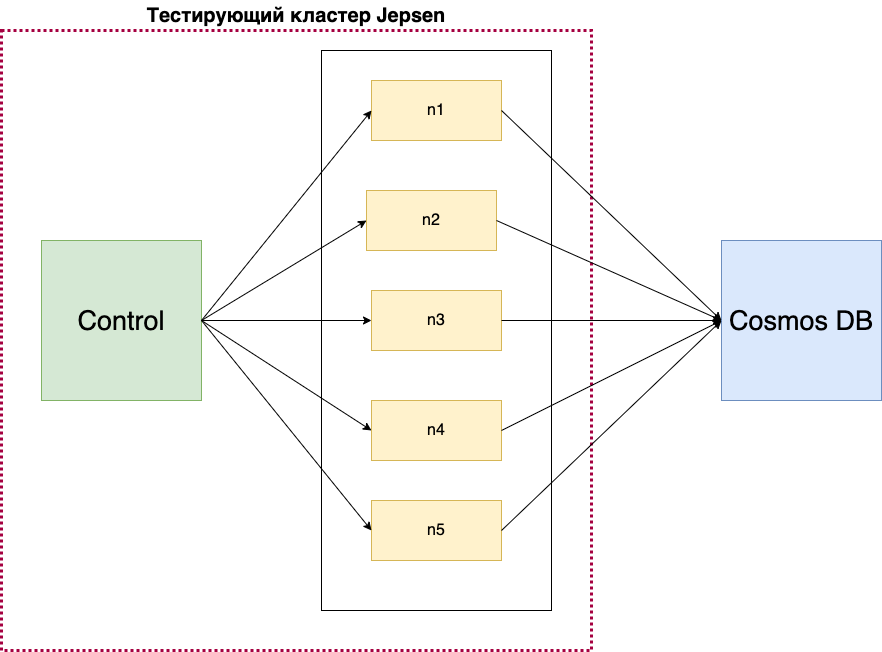
\includegraphics[width=\textwidth]{nodes-jepsen.png}
  \caption{Кластер тестирования Jepsen}
\end{figure}

\par В данном исследовании кластер Jepsen будет запущен на одном компьютере, используя docker compose. 
\subsubsection{Параметры компьютера}
\begin{itemize}
\item Операционная система --- macOS Big Sur версии $11.4$
\item Центральный процессор --- $2,3 GHz$ \textit{Dual-Core Intel Core i5}
\item Оперативная память --- $8 GB$
\item Количество ядер --- 2
\end{itemize}
Использование \textit{docker} упрощает и стандартизирует выполнение тестов. 
\par Репозиторий Jepsen предоставляет базовые настройки для запуска тестов в \textit{docker}: \underline{\href{https://github.com/jepsen-io/jepsen/tree/main/docker}{репозиторий с docker файлами}}.
\par Он поддерживает 2 вида контейнеров:  
\begin{itemize}
\item \textit{jepsen-control} --- управляет другими узлами, настройкой и удалением, генерирует данные и сбои;
\item \textit{jepsen-nX} --- один из узлов в кластере(будет использовано 5 таких узлов);
\end{itemize}

\section{Параметры базы данных}
Пропускная способность базы данных --- 1000 RU/s
\par \textit{RU (или EЗ)} --- англ. \textit{Request Unit},  единица запросов. 
\par ЕЗ — это единица производительности, которая абстрагирует системные ресурсы (например, ЦП, операции ввода-вывода в секунду и память), необходимые для выполнения операций базы данных, поддерживаемых Azure Cosmos DB.
\par Например, стоимость выполнения считывания(т. е. выборки одного элемента по его идентификатору и значению ключа раздела) для элемента размером 1 КБ составляет 1 единицу запроса (или 1 ЕЗ). Независимо от того, какие API вы используете для взаимодействия с контейнером Azure Cosmos и независимо от типа операции, затраты всегда измеряются в ЕЗ. 
\par Репликация данных --- включена, если задан специальный параметр теста \textit{--regions}. Тогда данные реплицируются в 3 региона, два региона на востоке США(\textit{East US}) и один регион в северной Европе(\textit{North Europe}).  Иначе хранится единственная реплика. 

\section{О реализации транзакций в Azure Cosmos DB}
\subsection{Транзакционный пакет(англ. \textit{TransactionalBatch})}
\subsubsection{Описание}
TransactionalBatch --- это, как утверждает документация, способ задания транзакции из нескольких операций (create, read, update, upsert, delete). Эти операции либо успешно выполнятся все вместе, либо завершатся сбоем.  В TransactionalBatch операции выполняются с одним и тем же ключом секции в контейнере.  Итак, если все операции выполняются успешно в том порядке, в котором они описаны в транзакционной пакетной операции, транзакция будет зафиксирована. Однако при сбое любой операции выполняется откат всей транзакции. 

\subsubsection{Тестирование}
Был запущен \textit{append} тест. \newline
Транзакции,  реализованные с помощью \textit{TransactionalBatch},  состояли из различных комбинаций двух операций: прочитать список значений по ключу \textit{id} и добавить новое уникальное целое число в список значений по ключу \textit{id}. Количество операций в одной транзакции было различное.
При тестировании использовались следующие параметры тестируемой системы:
\begin{itemize}
\item[] \textit{уровень согласованности} --- тестировалось на всех уровнях: строгий (англ.  \textit{strong}), ограниченное устаревание(англ.  \textit{bounded staleness}), сеанс(англ.  \textit{session}), постоянный префикс(англ.  \textit{consistent prefix}) и случайный(англ.  \textit{eventual})
\item[] \textit{количество потоков} --- 5
\item[] \textit{лимит времени на транзакцию} --- 60 секунд
\item[] \textit{ограничение на количество элементов по одному ключу} --- 256
\item[] \textit{максимальное количество операций в транзакции} --- 4
\item[] \textit{минимальное количество операций в транзакции} --- 1
\item[] \textit{репликация} --- отключена
\item[] \textit{сбои} --- без сбоев
\end{itemize}

\subsubsection{Результаты}
\par При тестировании транзакций с использованием TransactionalBatch Elle обнаружила следующие аномалии:
\begin{itemize}
\item внутренняя несогласованность (англ. \textit{internal inconsistency}) --- транзакция не соблюдает свои собственные предыдущие операции чтения и записи.
\item несогласованный порядок версий (англ.\textit{inconsistent version orders}) --- правила вывода предполагают циклический порядок обновления одного ключа.
\end{itemize}
Также, из отношений между аномалиями Elle\cite{Kingsbury2020ElleII} можно заключить, что из обнаружения в истории  \textit{inconsistent version orders} аномалии следует, что \textit{G1a} аномалия там также присутствует.
\par Кроме того, на уровнях \textbf{ограниченное устаревания} и \textbf{случайная} была обнаружена \textit{G2-item} аномалия. Обнаружение этой аномалии означает, что граф сериализации(\textit{DSG}) содержит направленный цикл с одним или несколькими ребрами анти зависимости \cite{IsolationLevelDefinitions}.
\par Транзакции, реализованные через \textit{TransactionalBatch}, теряют подтвержденные записи.  Кроме того, оказывается, что транзакции не изолированы. То есть, транзакции в такой реализации могли влиять на результаты других транзакций.
А значит, TransactionalBatch для \textbf{append} теста использовать нельзя. TransactionalBatch не удовлетворяет свойству внутренней консистентности транзакций.
\par Рассмотрим другой способ реализации транзакций в Cosmos DB. 

\subsection{Хранимые процедуры(англ. \textit{Stored procedures})}
Azure Cosmos DB предоставляет возможность транзакционного выполнение \textit{JavaScript} кода. При использовании API SQL в Cosmos DB можно реализовать триггеры, определяемые пользователем функции(\textit{UDF}) и хранимые процедуры.  Они пишутся на языке \textit{JavaScript}. 
\par Только операции над объектами из одного и того же раздела могут быть включены в одну транзакцию.  А значит, операции записи в разные контейнеры не могут быть выполнены транзакционно. 
\par Время выполнения одной хранимой процедуры ограничено пятью секундами.  И если транзакция длится дольше этого времени, то она будет отменена. Существует несколько способов для реализации <<долгоживущих>> транзакций через несколько обращений к серверу, но они нарушают атомарность.
\par Помимо того, что написанный JavaScript код будет выполняться атомарно, также данный способ реализации транзакций обещает хорошую производительность. Можно назвать следующие преимущества:
\begin{itemize}
\item \textit{пакетная обработка операций} --- группировка операций в пакеты и отправка этих пакетов. Это может сократить издержки на пересылку по сети и расходы на создание транзакций для отдельных операций; 
\item \textit{предварительная компиляция} --- определяемые пользователем функции, триггеры и хранимые процедуры заранее компилируются в байт-код.  Это позволяет хранимым процедурам работать быстро и занимать мало места.
\end{itemize}
\par
Хранимые процедуры и триггеры всегда выполняются на первичной реплике контейнера. 

\section{Реализация}
Для тестирования Cosmos DB был разработан \textit{append} тест c использованием транзакций, которые реализовывались через хранимые процедуры (англ. \textit{stored procedures}).  
\par Исходный код опубликован на \textit{github}: \newline 
\underline{\href{https://github.com/Alaska-666/jepsen.cosmos-db/tree/main}{https://github.com/Alaska-666/jepsen.cosmos-db/tree/main}}.

\section{Тестирование}
В этом параграфе будут описаны основные этапы тестирования Cosmos DB с помощью Jepsen. 
\par При запуске тестирующей системы Jepsen  выполнит настройку операционной системы на узлах \textit{jepsen-nX}. Будет использована \textit{jepsen.os.debian}.
\par Затем будет выполнено подключение к базе данных Cosmos DB, которая расположена <<в облаке>>. На этом этапе будет создан контейнер. В контейнере будут храниться пары ключ-значение,  где ключ есть уникальное целое число \textit{id}, а значение --- список целых чисел. 
\par Дальше на \textit{jepsen-control} узле будут генерироваться транзакции. Транзакции будут состоять из некоторого количества операций, где каждая операция это либо операция чтения списка чисел по ключу, либо добавление нового уникального целого числа в конец списка по ключу. 
\par Сгенерированные транзакции передаются на исполнение пять \textit{jepsen-nX}, где за их исполнение отвечает \textit{Client}. Транзакции применяются к тестируемой системе. Если операция чтения обращается к несуществующему ключу, то будет прочитан пустой список.  Если операция добавления обращается к несуществующему ключу, то создается список из одного элемента,  который нужно было добавить в конец.
\par При тестировании использовались транзакции минимум из одной операции и максимум --- из 20. Также использовались ограничения на количество чисел, которые могут быть записаны по одному \textit{id}. По умолчанию максимальная длина списка чисел --- 256.
\par После завершения работы \textit{client}-ов у Jepsen имеется список историй, где хранится также временная метка каждой операции и ее длительность.  Jepsen проводит проверку корректности историй с помощью Elle.  Elle строит граф сериализации для каждой истории, затем ищет циклы для выявления аномалий. 	

\subsection{Параметры тестирования}
Используемые параметры:
\begin{itemize}
\item[] \textit{уровень согласованности} --- тестировалось на всех уровнях
\item[] \textit{количество потоков} --- от 5 до 15
\item[] \textit{лимит времени на транзакцию} --- 60 секунд или 120 секунд
\item[] \textit{ограничение на количество элементов по одному ключу} --- 256 или 128
\item[] \textit{максимальное количество операций в транзакции} --- от 4 до 20
\item[] \textit{минимальное количество операций в транзакции} --- 1
\item[] \textit{репликация} --- отключена
\item[] \textit{сбои} --- сдвиг часов
\end{itemize}


\section{Результаты}
При тестировании Azure Cosmos DB, где транзакции реализованы с помощью хранимых процедур(англ. \textit{Stored procedures}), на всех уровнях согласованности(тесты запускались с разными параметрами, в том числе на разных уровнях согласованности: сильная, ограниченное устаревание, сеанс, префикс и случайная) были замечены G2-item  аномалии. 

\subsection{Обозначения для графиков}
Транзакции, изображенные на графиках аномалий, могут состоять из двух типов операций.
\subsubsection{Чтение (англ. \textit{read})}
\begin{figure}[H]
\centering
  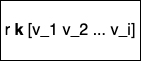
\includegraphics[scale=1.0]{images/read.png}
  \caption{Обозначение для операции чтения}
\end{figure}
Так будет обозначаться операция чтения в транзакции. \textit{r} --- операция чтения, \textit{\textbf{k}} --- \textit{id} объекта в таблице, который считывается. $[v_1 v_2 ... v_i]$ - сам объект, который был считан, массив целых чисел. Допускается, что может быть считан пустой массив, тогда он обозначается как $[]$.

\subsubsection{Добавление (англ. \textit{append})}
\begin{figure}[H]
\centering
  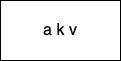
\includegraphics[scale=1.0]{images/append.png}
  \caption{Обозначение для операции добавления}
\end{figure}
Так будет обозначаться операция добавления нового элемента в транзакции. \textit{a} --- операция добавления, \textit{\textbf{k}} --- \textit{id} объекта в таблице,  к которому требуется добавить значение. \textit{v} - значение, добавляемое в конец массива целых чисел, который уже хранится.

\subsection{G2-item (англ. \textit{anti-dependency cycle}, цикл антизависимости)}
\subsubsection{\textit{Пример 1}}
\begin{figure}[H]
  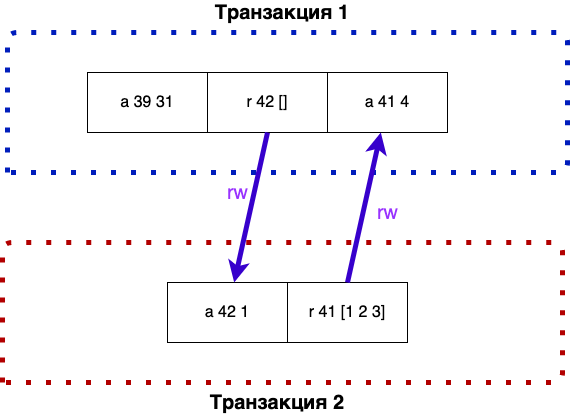
\includegraphics[width=\textwidth]{images/g2item1.png}
  \caption{G2-item}
\end{figure}

\par
Данная аномалия найдена при тестировании с использованием следующих параметров: 
\begin{itemize}
\item[] \textit{уровень согласованности} --- ограниченное устаревание(англ.  \textit{bounded staleness})
\item[] \textit{количество потоков} --- 15
\item[] \textit{лимит времени на транзакцию} --- 120 секунд
\item[] \textit{ограничение на количество элементов по одному ключу} --- 128
\item[] \textit{максимальное количество операций в транзакции} --- 4
\item[] \textit{репликация} --- отключена
\item[] \textit{сбои} --- нет
\end{itemize}

\textbf{Транзакция 1} выполняет операции:
\begin{enumerate}
\item добавление числа \textit{31} к массиву под \textit{id} \textit{\textbf{39}}
\item чтение массива значений по \textit{id} \textit{\textbf{42}} $\rightarrow$ получен пустой массив \textit{[ ]}
\item добавление числа \textit{4} к массиву под \textit{id} \textit{\textbf{41}}
\end{enumerate}

\textbf{Транзакция 2} выполняет операции:
\begin{enumerate}
\item добавление числа \textit{1} к массиву под \textit{id} \textit{\textbf{42}}
\item чтение массива значений по \textit{id} \textit{\textbf{41}} $\rightarrow$ получен массив $[1 2 3]$
\end{enumerate}

Ребро анти зависимости \textit{rw} добавляется между операцией 2 транзакции 1 и операций 1 транзакции 2 потому что операция 2 транзакции 1  считала некоторую(\textit{[ ]}) версию объекта с \textit{id} \textbf{42},  а операция 1 транзакции 2 изменила этот объект, добавив в массив значений новое число \textit{\textbf{1}}.  Также ребро анти зависимости \textit{rw} добавляется между операцией 2 транзакции 2 и операцией 3 транзакции 1, потому что операция 2 транзакции 2  считала некоторую(\textit{[1 2 3]}) версию объекта с \textit{id} \textbf{41},  а операция 3 транзакции 1 изменила этот объект, добавив в массив значений новое число \textit{\textbf{4}}.  В полученном графе сериализации наблюдается направленный цикл, содержащий 2 ребра анти зависимости. Значит, по определению, найдена \textit{G2-item} аномалия.

\par Эти две транзакции невозможно изолировать: если бы первая транзакция выполнялась первой, изолированно, ее запись с \textit{id} 41 была бы видна второй транзакции --- и наоборот. Но поскольку эти транзакции не записывались в один и тот же \textit{id}, им разрешено (при \textbf{изоляции моментальных снимков}) выполняться одновременно.

\subsubsection{\textit{Пример 2}}
\begin{figure}[H]
  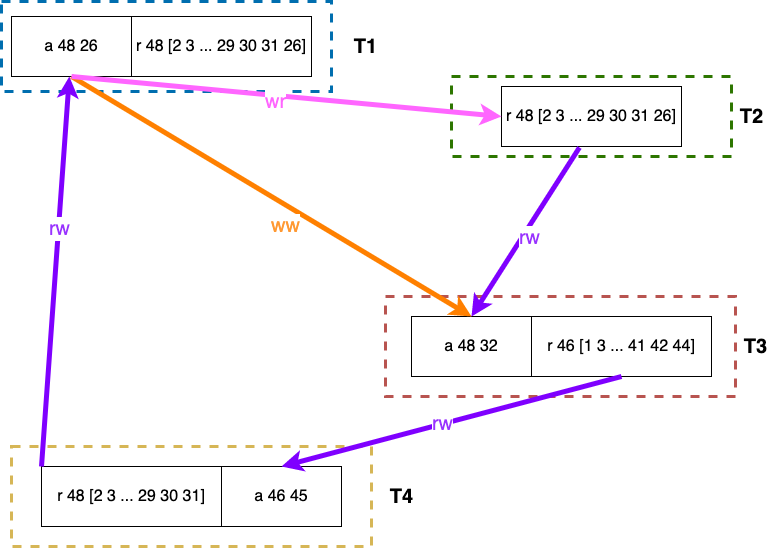
\includegraphics[width=\textwidth]{images/g2item2.png}
  \caption{G2-item}
\end{figure}

\par Данная аномалия найдена при тестировании с использованием следующих параметров: 
\begin{itemize}
\item[] \textit{уровень согласованности} --- постоянный префикс(англ.  \textit{consistent prefix})
\item[] \textit{количество потоков} --- 15
\item[] \textit{лимит времени на транзакцию} --- 120 секунд
\item[] \textit{ограничение на количество элементов по одному ключу} --- 128
\item[] \textit{максимальное количество операций в транзакции} --- 7
\item[] \textit{репликация} --- отключена
\item[] \textit{сбои} --- нет
\end{itemize}

Это более сложный цикл, состоящий из 4 транзакций.  Каждая из этих транзакций зависит от другой.  \par

Транзакция 1(\textbf{$T_1$}) выполняет операции:
\begin{enumerate}
\item добавление числа \textit{26} к массиву под \textit{id} \textit{\textbf{48}}
\item чтение массива значений по \textit{id} \textit{\textbf{48}} $\rightarrow$ получен массив \textit{[2 3 4 5 6 7 8 9 1 10 11 12 13 14 15 16 17 18 19 20 21 22 23 25 27 28 29 30 31 26]}
\end{enumerate}

\par Транзакция 2(\textbf{$T_2$}) выполняет операцию:
\begin{enumerate}
\item чтение массива значений по \textit{id} \textit{\textbf{48}} $\rightarrow$ получен массив \textit{[2 3 4 5 6 7 8 9 1 10 11 12 13 14 15 16 17 18 19 20 21 22 23 25 27 28 29 30 31 26]}
\end{enumerate}

\par Транзакция 3(\textbf{$T_3$}) выполняет операции:
\begin{enumerate}
\item добавление числа \textit{32} к массиву под \textit{id} \textit{\textbf{48}}
\item чтение массива значений по \textit{id} \textit{\textbf{46}} $\rightarrow$ получен массив \textit{[1 3 4 5 6 2 8 9 10 7 11 13 12 14 15 17 21 22 18 19 16 23 24 25 26 27 29 30 31 20 33 36 35 32 28 34 38 37 39 40 41 42 44]}
\end{enumerate}

\par Транзакция 4(\textbf{$T_4$}) выполняет операции:
\begin{enumerate}
\item чтение массива значений по \textit{id} \textit{\textbf{48}} $\rightarrow$ получен массив \textit{[2 3 4 5 6 7 8 9 1 10 11 12 13 14 15 16 17 18 19 20 21 22 23 25 27 28 29 30 31]}
\item добавление числа \textit{45} к массиву под \textit{id} \textit{\textbf{46}}
\end{enumerate}

Далее обозначение \textbf{$T_1$}.1 означает операцию 1 транзакции 1.  

\par \textbf{Ребра:}
\begin{itemize}
\item \textit{rw} --- \textbf{$T_4$}.1 $ \xrightarrow{\textit{rw}}$  \textbf{$T_1$}.1,  так как \textbf{$T_4$}.1 считывает массив по $id=48$ и получает массив значений без числа $26$, а \textbf{$T_1$}.1 изменяет массив, добавляя в него новое число $26$;
\item \textit{rw} --- \textbf{$T_2$}.1 $ \xrightarrow{\textit{rw}}$  \textbf{$T_3$}.1,  так как \textbf{$T_2$}.1 считывает массив по $id=48$ и получает массив значений без числа $32$, а \textbf{$T_3$}.1 изменяет массив, добавляя в него новое число $32$;
\item \textit{rw} --- \textbf{$T_3$}.2 $ \xrightarrow{\textit{rw}}$  \textbf{$T_4$}.2,  так как \textbf{$T_3$}.2 считывает массив по $id=46$ и получает массив значений без числа $45$, а \textbf{$T_4$}.2 изменяет массив, добавляя в него новое число $45$;
\item \textit{ww} --- \textbf{$T_1$}.1 $ \xrightarrow{\textit{ww}}$  \textbf{$T_3$}.1, так как транзакции изменяют один и тот же объект $id=48$, одна транзакция добавляет число $26$, а другая $32$;
\item \textit{wr} --- \textbf{$T_1$}.1 $ \xrightarrow{\textit{wr}}$  \textbf{$T_2$}.1, так как \textbf{$T_2$}.1 считала массив значений объекта $id=48$ и в массиве содержалось число $26$, добавленное транзакцией \textbf{$T_1$}.1.
\end{itemize}
В полученном графе сериализации наблюдается направленный цикл, содержащий 3 ребра анти зависимости. Значит, по определению, найдена \textit{G2-item} аномалия.
\par Если пытаться упорядочить данные транзакции, то наблюдается следующее поведение($T_i<T_j$ --- транзакция $T_i$ произошла раньше $T_j$):
\begin{itemize}
\item $T_2 < T_3$, так как $T_2$ не наблюдает число $32$, добавленное в транзакции $T_3$; 
\item $T_3 < T_4$, так как $T_3$ не наблюдает число $45$, добавленное в транзакции $T_4$; 
\item $T_4 < T_1$, так как $T_4$ не наблюдает число $26$, добавленное в транзакции $T_1$;
\item $T_1 < T_2$, так как $T_2$ наблюдает число $26$, добавленное в транзакции $T_1$.  
\end{itemize}
Получили противоречие. Эти четыре транзакции невозможно изолировать.

\subsection{Анализ результатов}
 \textit{G2-item} аномалия не редкость. Примерно в 15\% транзакций наблюдались аномалии во время нормальной работы, без сбоев.
\par В документации Azure Cosmos DB сказано, что поддерживаемый уровень изоляции транзакций --- \textbf{изоляция моментальных снимков}. 
\par При \textit{изоляция моментальных снимков} транзакциям, которые не записывают в один и тот же \textit{id},  разрешено выполняться одновременно.  То есть, полученные  истории, по-видимому, не нарушают \textit{изоляцию моментальных снимков}, но, тем не менее, демонстрируют циклические зависимости транзакций.
\par База данных Azure Cosmos DB соответствует заявленному уровню изоляции.

\chapter{Заключение}
В данной работе был обозначен ряд проблем, которые возникают в распределенных системах. Зачастую они являются результатом сочетания маловероятных событий. Также их сложно выявить на этапе разработки распределенной системы.  Это обуславливает необходимость введения формальных определений различных моделей согласованности.
\par Также сложность обнаружения различных нарушений изоляции обуславливает появление Jepsen как инструмента для проверки гарантий выполнения важнейших свойств распределенных систем. Этот инструмент был представлен в данной работе.
\par Кроме того, в этой работе с помощью Jepsen была проанализирована реальная база данных --- Cosmos DB.  Cosmos DB утверждает, что поддерживает изоляцию моментальных снимков как уровень изоляции транзакций. Однако использование этих транзакций осложняется запутанной документацией и API.  В процессе тестирования наблюдались истории, которые казались совместимыми с изоляцией моментальных снимков, но также включали аномалии G2-item (циклы анти зависимости), в которых транзакции не наблюдали эффектов друг друга.  Такие аномалии были замечены в 15\% историй.  Такое поведение корректно при изоляции моментальных снимков.  А значит,  база данных Azure Cosmos DB соответствует заявленному уровню изоляции.
\par Итак, в этой работе было проведено лишь краткое исследование. В дальнейшем в рамках развития данной работы возможно реализовать другие тесты, например, \textit{register} тест, а также исследовать поведение базы данных при различных сбоях.


\bibliographystyle{unsrt}
\bibliography{references}


\end{document}
